\chapter{Analysis Software}
\label{app:Software}

The analysis conducted in this thesis requires processing large amounts of data, both as additional datasets arrive from CERN, and also repeatedly as analysis needs develop. It is thus crucial that the software used to process the data performs efficiently, allowing the analysis to progress rapidly without too much computational delay. To achieve this, a three-tier ecosystem was developed in C++, based on standard CERN software. 

\section{RutgersAODReader}
The CMS experiment provides measurement data and simulated samples in the so-called MiniAOD format. This format can be decoded using the CMSSW software \cite{CMSSW} which is built on top of the ROOT data analysis framework \cite{Brun:1997pa} and also provided by CMS.

RutgersAODReader interfaces with CMSSW to extract event information from measurement data and simulated samples which is then used to create simple collections of objects that are associated with particles reconstructed by the detector. Those collections, also called ``products'', are stored along with a few basic analysis variables like \MET in so-called flat ntuple files using the standard ROOT file format.

\section{EventAnalyzer}
\label{app:Software/EventAnalyzer}
EventAnalyzer uses RutgersAODReader's flat ntuple output files as input. It then proceeds with higher-level computations, such as calculating isolation and other object-specific variables (see Sec.~\ref{sec:Selection/Object}), and creating collections of reconstructed particles with additional selection criteria such as collections of ``good muons'' and ``good electrons'' which fulfill the analysis requirements (isolation, promptness, etc.). The software also provides capabilities to make sure that objects do not overlap; for example, one can discard electrons that are too close to a reconstructed muon. Furthermore, particles can be reassigned to collections of another type, as is needed for the implementation of our fake rate method (see Sec.~\ref{sec:bkg_fakeLight/Method}). Fig.~\ref{fig:EventAnalyzer} displays an overview of the various object collections used.

\begin{figure}
\begin{center}
	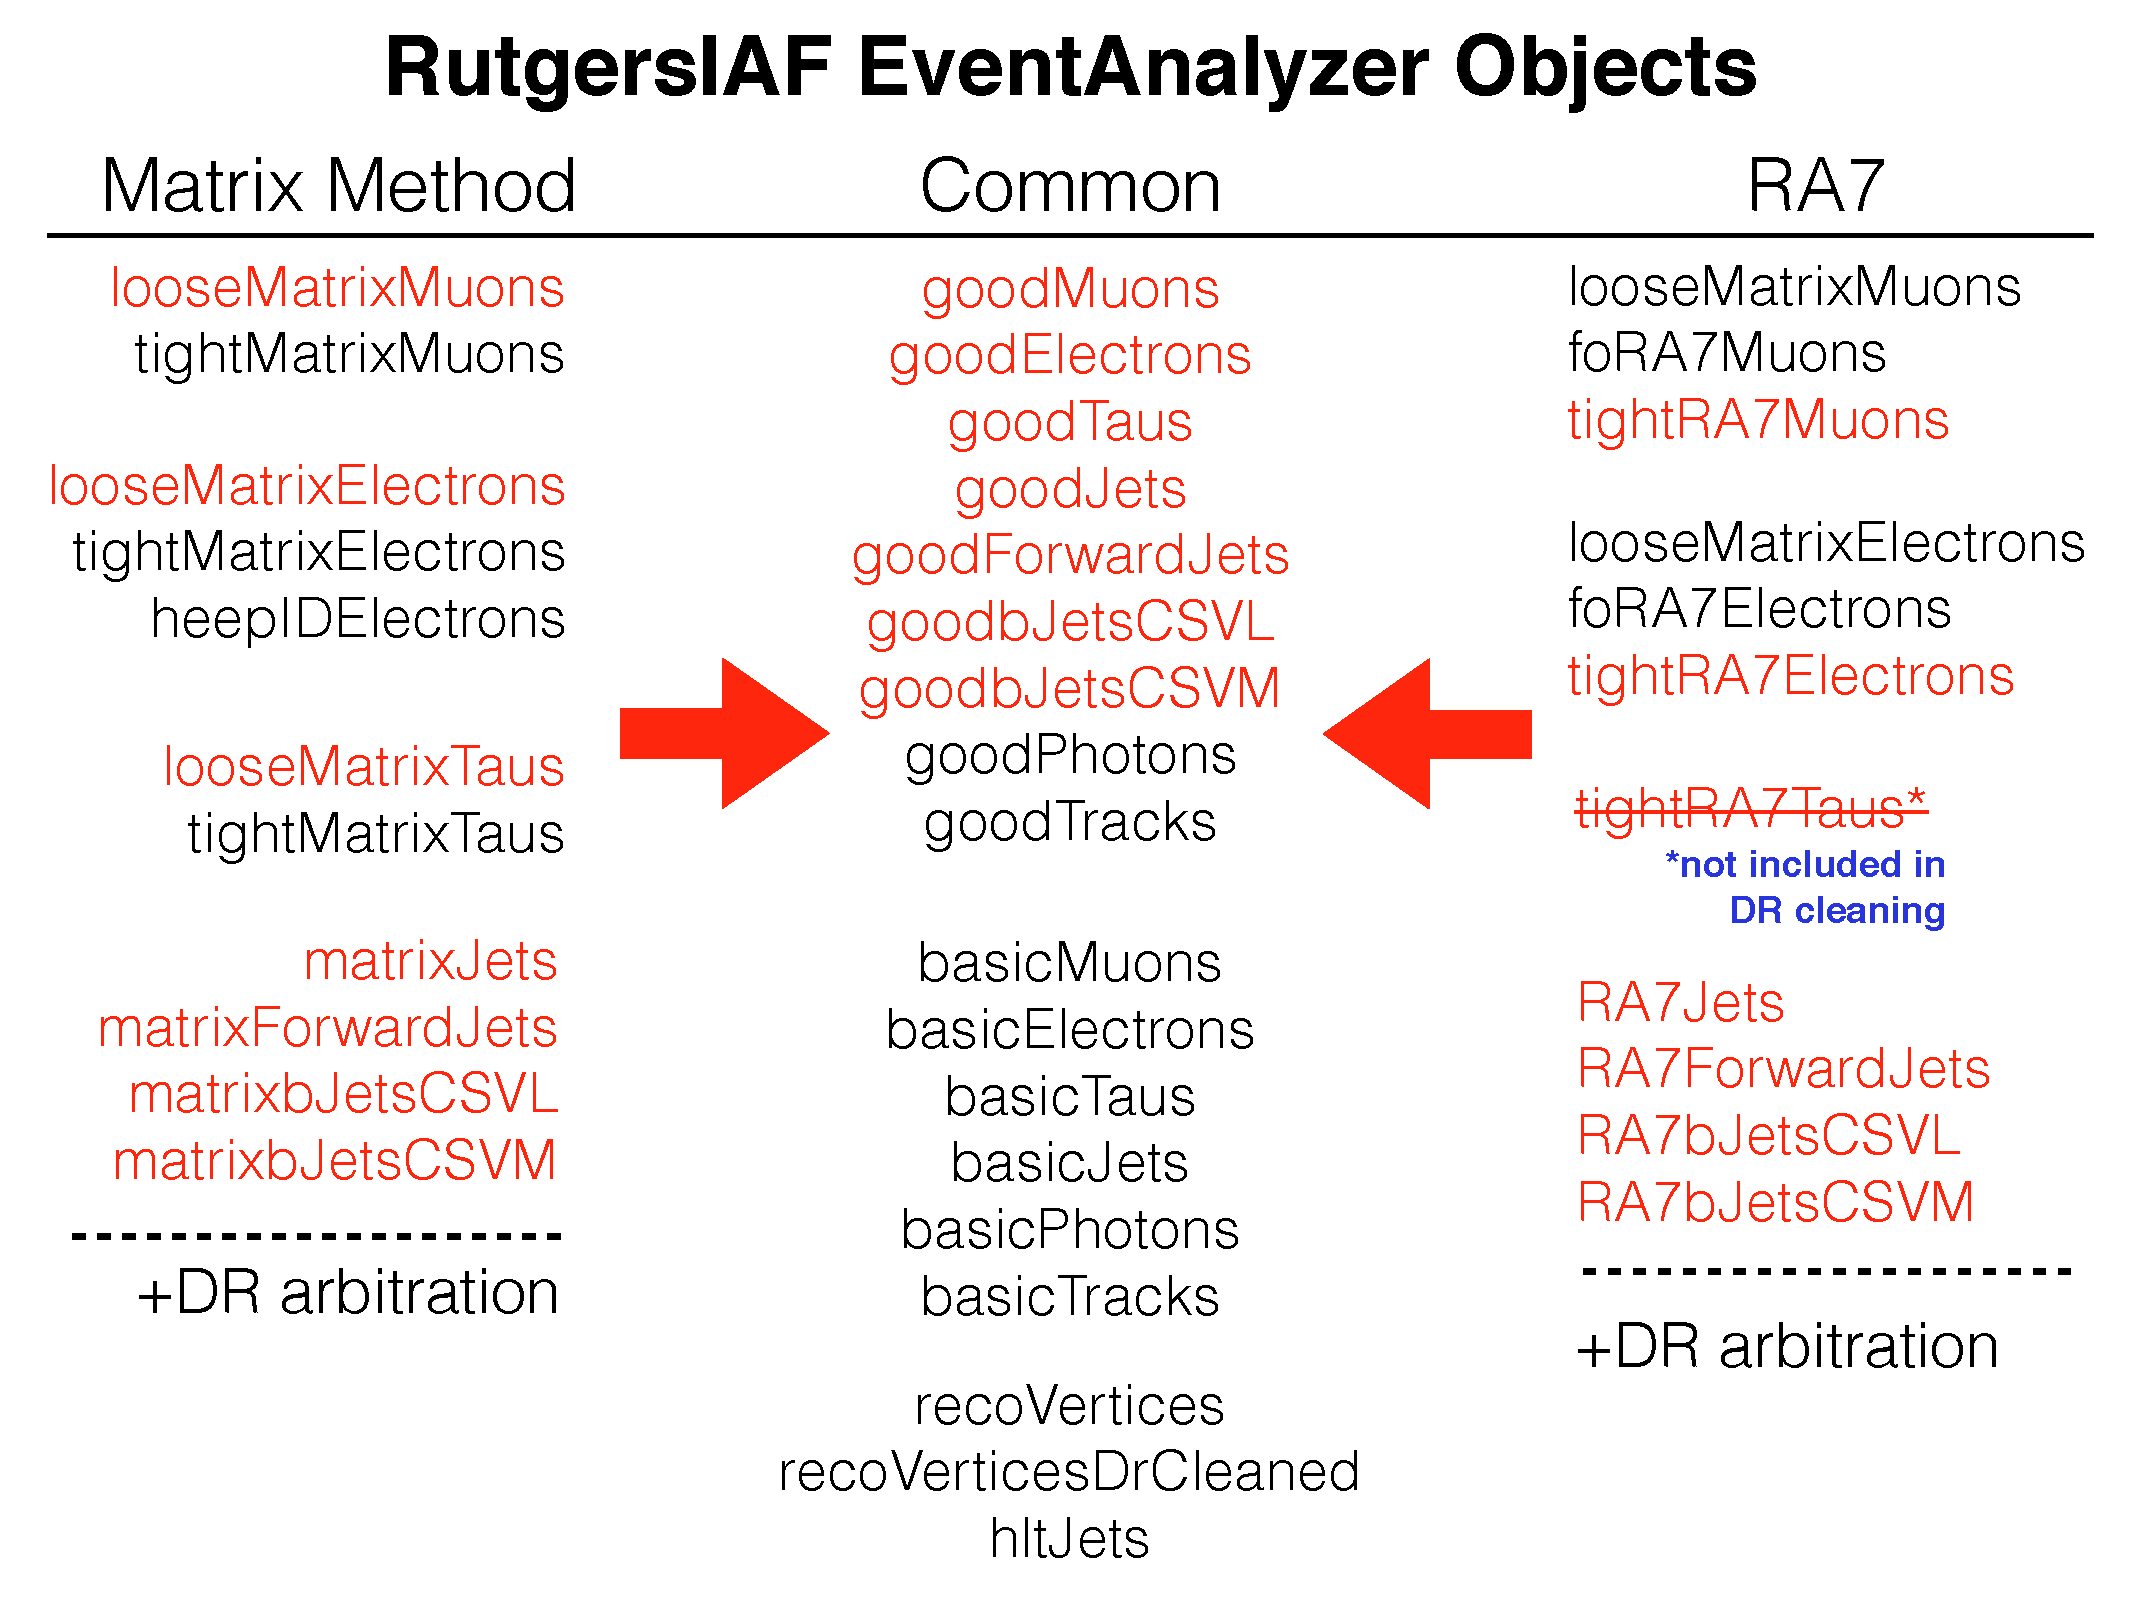
\includegraphics[width=\textwidth]{Appendix/EventAnalyzer}
	\caption{Overview of the object collections used in EventAnalyzer.
	\label{fig:EventAnalyzer}}
\end{center}
\end{figure}

After calculating all the ``object variables'' which relate to a specific reconstructed particle, additional ``event variables'' are computed. Those are properties of the event and not of specific objects, e.\,g. the number of leptons passing all quality requirements, or whether an event contains an OSSF lepton pair whose invariant mass is consistent with a \Z boson decay (see Sec.~\ref{sec:Strategy/general}).

The categorization of data, background, and signal events into signal and control regions is usually based on such event variables. While EventAnalyzer provides several output mechanisms\hairspace{}---\hairspace{}from condensed histograms to full event dumps\hairspace{}---, the so-called AnalysisTree output format is used in most cases. This format is based on the standard ROOT file format and contains all computed event variables in a way that is easily accessible subsequently, either directly from the ROOT command prompt, or from within additional software that reads AnalysisTree files. Special storage mechanisms for boolean event variables and certain event weights are, however, incompatible with standard ROOT tools such as \texttt{hadd} (used for combining multiple files) and require custom variants of these tools (specifically, \texttt{haddR}).

All of EventAnalyzer's actions are configured through a configuration file. The EventAnalyzer engine itself is agnostic of the specific type of physics that is being investigated, but it understands concepts such as particle collections, momentum vectors, spatial distance, or invariant mass. The configuration file is used to specify which particles are to be related in which ways, and allows to declare variables for storage that are of interest on the analysis level such as the scalar sum of lepton transverse momenta, $L_\textrm{T}$. It also allows to specify the output format as well as skimming criteria in order to save on storage and processing time.

\section{AnalysisPresenter}
\subsection{Scope and Design Principles}
Once all data, background, and signal samples have been made available in AnalysisTree format, AnalysisPresenter is used to categorize events, apply event weights (such as pile-up, \pt, or $n_\textrm{jets}$ corrections), estimate the data-driven fake backgrounds by applying fake rates (including any parameterizations that may have been defined) to the seed samples (see Sec.~\ref{sec:bkg_fakeLight}), and scale MC backgrounds and signal to the data luminosity.

These scalings are performed on the fly at the time of reading events from the AnalysisTree input files. For each sample that is read in, a multidimensional histogram is created in memory which is filled using weights as prescribed by the scalings. Just like EventAnalyzer, the AnalysisPresenter engine is unaware of the physics that is being considered. Instead, the user needs to specify the variables of interest and the binning scheme through a configuration file. The axes of the multidimensional histogram are constructed based on these specifications and can later be used for cutting and binning. An axis can either be any event variable stored in the AnalysisTree, or a combination thereof. Simple combinations can be declared inline, while more complicated functions (such as a hash of the event number) require resorting to a user-defined C++ function from within the axis specification. Statistical uncertainties are stored with each bin that is populated.

AnalysisPresenter also allows modeling systematic uncertainties for backgrounds and signal. Correlations and anti-correlations can be modeled both between samples (e.\,g. the luminosity uncertainty for rare backgrounds estimated from MC, and for signal) as well as between bins within the same sample (e.\,g. bin migration due to \MET uncertainties). To keep track of these details for every sample, a copy of the multidimensional histogram is filled for each systematic uncertainty and sample, with a variation by one standard deviation applied. By subtracting the nominal histogram, the absolute impact of the systematic uncertainty can be determined; the sign distinguishes anti-correlations from correlations. Systematic uncertainties are specified either as a percentage number, as a formula that depends on arbitrary event variables or user-defined functions, or by declaring that an event variable be replaced by another one in order to evaluate the changes in how the multidimensional histogram is populated.

\subsection{Distributions}
Simple distributions like the $L_\textrm{T} + \MET$ distributions in Fig.~\ref{fig:Optimization2} can be made in a straightforward manner from the multidimenstional histograms: First, cuts are applied by setting an ``axis range'', e.g. $3 \leq n_\textrm{leptons} \leq 4$ to require three or four leptons. This can be thought of as slicing out a subset of the multidimensional histogram. Second, a projection is taken onto the axis of interest, e.\,g.  $L_\textrm{T} + \MET$. When projecting, the histogram is collapsed into a one-dimensional histogram along the projection axis; bins along all other dimensions are integrated. Statistical uncertainties are added in quadrature; systematic uncertainties are taken care of by repeating the slicing and projection steps with the correspondong copies of the multidimensional histograms.

The projection method returns an object that offers various ways to output the resulting distributions, for example as a plot like those in Fig.~\ref{fig:Optimization2}, or as an ASCII table. Within each projection object, an event list is stored along with the data, background, and signal histograms. This allows for easy investigation of interesting events.

\subsection{Bundling Mechanism and MC Subtraction}
As described in Sec.~\ref{sec:Samples/Signal}, the signal consists of 27 different processes which we generate separately. It is desirable that those samples are summed up and displayed together. Similarly, one might want the combine several rare backgrounds into one, to avoid visual clutter. For this purpose, AnalysisPresenter supports the bundling of samples. The bundling is performed after cutting and projecting has been done.

The bundling mechanism may not only be used for presentation purposes, but also for physical purposes. Our fake rate method, for example, requires subtracting an overlapping prediction from the \ttbar MC simulation. This can be handled by declaring the overlapping \ttbar background estimate as an additional background process in the AnalysisPresenter configuration file, but with a negative weight. This estimate can then be bundled with the fake background prediction itself; the negative weights for the \ttbar component will effect the desired subtraction. The result is what's labeled the ``TrackFakes'' component in Fig.~\ref{fig:fakeLight_Z_MOSSF}.

Samples of single physics processes share the same C++ interface as bundles of processes. This means that bundles may in turn be bundled up with other processes or bundles. For example, the ``Misidentified'' component in Fig.~\ref{fig:WZ} is a bundle of the ``TrackFakes'' and the ``PhotonFakes'' bundle. The summation is done for visual purposes only.

As we have seen, it is desirable to allow histogram bins to assume negative values for the purposes of MC subtraction through the bundling mechanism. Another use case of negative bin contents is when an MC generator such as MadGraph5\_aMC@NLO \cite{Alwall:2011uj} provides negative weights for some events. For bins in the tail of an event variable distribution, it may then happen that they are predominantly populated by events with negative weights. This is usually an artifact of the fact that the multidimensional histograms are extremely finely binned: Upon projection on any axis, the other axes are integrated over, so that the result is usually positive. It is thus important to keep the negative bins in the multidimensional histogram; discarding them would bias the histogram integral to higher average values when the binning scheme is replaced by a more granular one. Only after a projection is done, the user may want to enforce that negative bin contents be replaced by zero to make sure predictions are physical.

Thus, for each contribution (be it bundled or not), the user may specify whether bin contents should be bounded by 0 from below, depending on whether the contribution is intended to be used for subtraction purposes via the bundling mechansism or not.

\subsection{Channel Collections and Datacards}
A set of cuts (axis ranges) can be frozen into a ``channel''. Channels share the same C++ interface as projections; in particular, they can be output as a plot or a table.

In addition, multiple channels can be combined into a structure called ``channel collection''. From this structure, AnalysisPresenter can create a so-called datacard which contains information on observation, signal, background composition of all the channels involved, as well as statistical and systematic uncertainties including their correlations. The datacard format is compatible with the standard CMS statistics tools and can be used for statistical interpretation of the analysis, as is done in Sec.~\ref{sec:Interpretation}.

When creating a datacard, the bundling prescriptions are observed. This is not only important for purposes of MC subtraction, but also useful to limit the level of detail in the datacard in order to reduce the runtime of the statistical interpretation (e.\,g. to combine rare backgrounds). Furthermore, it is enforced that the channels within a channel collection do not have duplicate events, that is, they are exclusive.

\subsection{Runtime}
AnalysisPresenter is mainly a categorization tool, but does not actually calculate sophisticated physical quantities like invariant masses. (This is the task of EventAnalyzer, see Sec.~\ref{app:Software/EventAnalyzer}). It therefore can populate its main data structures\hairspace{}---\hairspace{}the multidimensional histograms\hairspace{}---\hairspace{}at a rate of about 20000 events per second. Nevertheless, the bulk of the processing time comes from reading events from the samples (between a few seconds and several minutes, depending on the use case).

Cuts, projections, bundlings, as well as channel collection and datacard creation are then performed within a fraction of second. Since it is possible to change the cuts at runtime, various types of output can be created for different selections without rereading the samples. Thus, if the user plans ahead and declares all axes that are intended to be used for cutting and binning, changes to the analysis selection can be studied very quickly in various regions. The runtime is roughly proportional to the number of samples and to the number of systematic uncertainties declared, and also depends on the binning granularity, as the bookkeeping overhead increases with the number of bins.
